\subsection{Experiment A: Controlled Repeated-Instance Scaling}
\label{subsec:experiment-a}
Experiment A uses four helicopters and four demand areas, with 20, 30, 40,
50 and 60 tasks and 30 generated instances per size. Each instance is solved
by Greedy Benefit and Greedy Density, and by HiGHS without a start, with a
Benefit start, and with a Density start. The three MILP variants share the
same matrix and solver settings. Each receives independent solve allowances
of 1, 5, 15, 60 and 600 s. The 600-s runs provide the main comparison below;
the shorter budgets are examined in Section~4.3.
The multidimensional benefit defined in Section~3.3 is
used throughout.

\begin{figure}[!htbp]
\centering
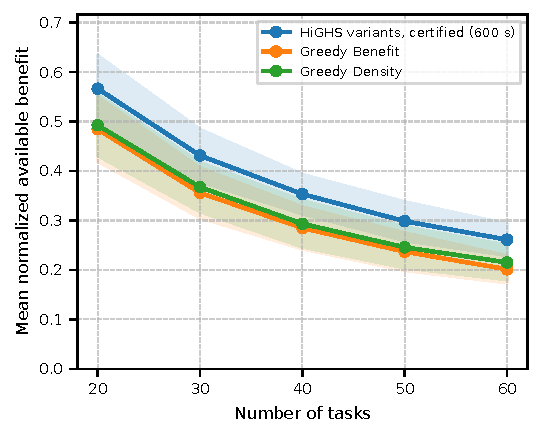
\includegraphics[width=\columnwidth]{A1_solution_quality_coverage_aware.pdf}
\caption{Normalized available benefit in Experiment A at the 600-s MILP
allowance. Lines denote means over the same 30 instances at each task count;
shaded regions denote one sample standard deviation. An externally available
idle plan is scored as zero when cold returns no incumbent. The three MILP curves coincide and are drawn once because all three variants certified every instance and their paired benefits agree within numerical tolerance. }
\label{fig:expA-quality}
\end{figure}

At 600 s, cold HiGHS certified 150/150 instances; the Benefit and Density starts certified 150/150 and 150/150, respectively. For Greedy Benefit, mean paired shortfalls ranged from 14.4\% to 22.9\%. For Greedy Density, mean paired shortfalls ranged from 13.0\% to 17.9\%. Shortfall calculations use the 150/150 instances with a certified reference from this objective and model; unknown optima are excluded.

\begin{figure*}[!htbp]
\centering
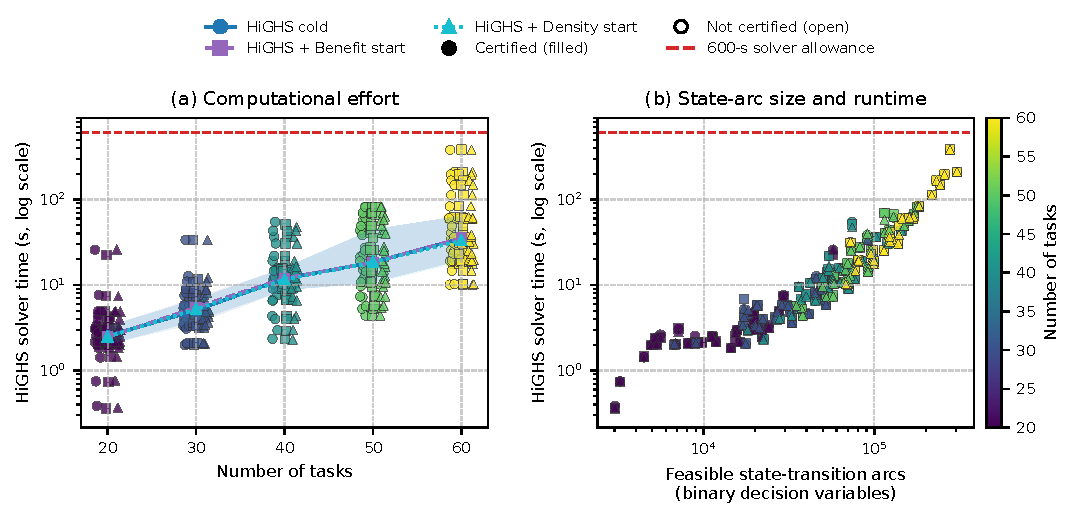
\includegraphics[width=\textwidth]{A8_computational_effort.pdf}
\caption{Experiment A computational effort for the three initialization
strategies. Panel (a) shows all solver times, with medians and interquartile
ranges. Panel (b) relates solver time to generated state-transition arcs.
Marker shape identifies the initialization strategy; filled and open markers
denote certified and uncertified runs. The dashed line is the 600-s solver
allowance. Table~\ref{tab:expA-runtime} reports end-to-end time, including
preparation.}
\label{fig:expA-effort}
\end{figure*}

On pairs where both variants certified, median warm-minus-cold end-to-end changes were HiGHS + Benefit start: +0.03 s over 150 matched certified pairs; HiGHS + Density start: +0.02 s over 150 matched certified pairs. Positive changes mean that the warm variant took longer. 
Warm-start availability by itself does not establish a search improvement:
the constructive plan is already available before optimization. The budget
analysis therefore also compares each warm result with cold retaining the
same greedy plan as an external fallback.

\begin{table}[!htbp]
\centering
\caption{Experiment A: solution quality and certification at the 600-s MILP budget.}
\label{tab:expA-quality}
\scriptsize
\setlength{\tabcolsep}{2.6pt}
\renewcommand{\arraystretch}{1.08}
\begin{tabular}{@{}ccccc@{}}
\toprule
Tasks & \makecell{Normalized available\\benefit\\Mean $\pm$ SD} & \makecell{Completed tasks\\Mean $\pm$ SD} & \makecell{Certified\\runs} & \makecell{Shortfall\\(\%)} \\
\midrule
\multicolumn{5}{@{}l}{\textit{Panel A: HiGHS cold}}\\
\addlinespace[0.2em]
20 & $0.5662 \pm 0.0674$ & $13.93 \pm 1.74$ & $30/30$ & 0.0 \\
30 & $0.4311 \pm 0.0530$ & $16.23 \pm 1.72$ & $30/30$ & 0.0 \\
40 & $0.3531 \pm 0.0402$ & $18.00 \pm 1.82$ & $30/30$ & 0.0 \\
50 & $0.2984 \pm 0.0396$ & $19.17 \pm 2.05$ & $30/30$ & 0.0 \\
60 & $0.2610 \pm 0.0324$ & $20.07 \pm 2.41$ & $30/30$ & 0.0 \\
\midrule
\multicolumn{5}{@{}l}{\textit{Panel B: Greedy Benefit}}\\
\addlinespace[0.2em]
20 & $0.4843 \pm 0.0651$ & $13.63 \pm 1.38$ & -- & 14.4 \\
30 & $0.3557 \pm 0.0507$ & $15.67 \pm 1.52$ & -- & 17.4 \\
40 & $0.2847 \pm 0.0427$ & $16.83 \pm 1.88$ & -- & 19.5 \\
50 & $0.2367 \pm 0.0383$ & $17.33 \pm 2.14$ & -- & 20.7 \\
60 & $0.2012 \pm 0.0278$ & $17.90 \pm 2.11$ & -- & 22.9 \\
\midrule
\multicolumn{5}{@{}l}{\textit{Panel C: Greedy Density}}\\
\addlinespace[0.2em]
20 & $0.4923 \pm 0.0618$ & $13.97 \pm 1.38$ & -- & 13.0 \\
30 & $0.3672 \pm 0.0499$ & $16.17 \pm 1.51$ & -- & 14.7 \\
40 & $0.2932 \pm 0.0472$ & $17.50 \pm 1.94$ & -- & 17.2 \\
50 & $0.2456 \pm 0.0419$ & $19.10 \pm 2.29$ & -- & 17.9 \\
60 & $0.2151 \pm 0.0353$ & $19.97 \pm 2.14$ & -- & 17.8 \\
\midrule
\multicolumn{5}{@{}l}{\textit{Panel D: HiGHS + Benefit start}}\\
\addlinespace[0.2em]
20 & $0.5662 \pm 0.0674$ & $13.93 \pm 1.74$ & $30/30$ & 0.0 \\
30 & $0.4311 \pm 0.0530$ & $16.23 \pm 1.72$ & $30/30$ & 0.0 \\
40 & $0.3531 \pm 0.0402$ & $18.00 \pm 1.82$ & $30/30$ & 0.0 \\
50 & $0.2984 \pm 0.0396$ & $19.17 \pm 2.05$ & $30/30$ & 0.0 \\
60 & $0.2610 \pm 0.0324$ & $20.07 \pm 2.41$ & $30/30$ & 0.0 \\
\midrule
\multicolumn{5}{@{}l}{\textit{Panel E: HiGHS + Density start}}\\
\addlinespace[0.2em]
20 & $0.5662 \pm 0.0674$ & $13.93 \pm 1.74$ & $30/30$ & 0.0 \\
30 & $0.4311 \pm 0.0530$ & $16.23 \pm 1.72$ & $30/30$ & 0.0 \\
40 & $0.3531 \pm 0.0402$ & $18.00 \pm 1.82$ & $30/30$ & 0.0 \\
50 & $0.2984 \pm 0.0396$ & $19.17 \pm 2.05$ & $30/30$ & 0.0 \\
60 & $0.2610 \pm 0.0324$ & $20.07 \pm 2.41$ & $30/30$ & 0.0 \\
\bottomrule
\end{tabular}
\begin{minipage}{0.98\columnwidth}
\footnotesize
Means and sample SD summarize the same instances for all five variants. All MILP variants receive 600 s. Shortfalls are computed per instance against a certified optimum of the same model and objective, then averaged; unknown optima are excluded. Every generated instance has a certified reference. Certification denotes HiGHS optimal status at relative MIP tolerance 1e-06; it is not applicable to the greedy policies.
\end{minipage}
\end{table}

\begin{table}[!htbp]
\centering
\caption{Experiment A: computational performance and generated state-arc MILP size.}
\label{tab:expA-runtime}
\scriptsize
\setlength{\tabcolsep}{2.4pt}
\renewcommand{\arraystretch}{1.08}
\begin{tabular}{@{}ccccc@{}}
\toprule
Tasks & \makecell{Runtime\\Mean $\pm$ SD} & \makecell{Maximum\\runtime} & \makecell{Variables\\mean} & \makecell{Constraints\\mean} \\
\midrule
\multicolumn{5}{@{}l}{\textit{Panel A: HiGHS cold (seconds)}}\\
\addlinespace[0.2em]
20 & $3.65 \pm 4.47$ & $26.13$ & 14{,}939 & 6{,}012 \\
30 & $6.56 \pm 5.85$ & $34.25$ & 32{,}661 & 11{,}697 \\
40 & $15.39 \pm 11.97$ & $55.15$ & 60{,}015 & 18{,}937 \\
50 & $29.67 \pm 24.37$ & $83.38$ & 92{,}362 & 25{,}682 \\
60 & $69.54 \pm 80.82$ & $382.53$ & 144{,}561 & 34{,}880 \\
\midrule
\multicolumn{5}{@{}l}{\textit{Panel B: Greedy Benefit (milliseconds)}}\\
\addlinespace[0.2em]
20 & $1.327 \pm 1.525$ & $9.367$ & -- & -- \\
30 & $1.316 \pm 0.110$ & $1.735$ & -- & -- \\
40 & $1.623 \pm 0.146$ & $2.044$ & -- & -- \\
50 & $1.890 \pm 0.159$ & $2.386$ & -- & -- \\
60 & $2.160 \pm 0.143$ & $2.428$ & -- & -- \\
\midrule
\multicolumn{5}{@{}l}{\textit{Panel C: Greedy Density (milliseconds)}}\\
\addlinespace[0.2em]
20 & $0.896 \pm 0.060$ & $1.049$ & -- & -- \\
30 & $1.147 \pm 0.064$ & $1.288$ & -- & -- \\
40 & $1.449 \pm 0.127$ & $1.802$ & -- & -- \\
50 & $1.762 \pm 0.183$ & $2.280$ & -- & -- \\
60 & $2.123 \pm 0.184$ & $2.550$ & -- & -- \\
\midrule
\multicolumn{5}{@{}l}{\textit{Panel D: HiGHS + Benefit start (seconds)}}\\
\addlinespace[0.2em]
20 & $3.47 \pm 3.89$ & $22.76$ & -- & -- \\
30 & $6.68 \pm 5.79$ & $34.29$ & -- & -- \\
40 & $15.27 \pm 11.54$ & $51.29$ & -- & -- \\
50 & $29.90 \pm 24.62$ & $83.49$ & -- & -- \\
60 & $69.75 \pm 81.12$ & $385.03$ & -- & -- \\
\midrule
\multicolumn{5}{@{}l}{\textit{Panel E: HiGHS + Density start (seconds)}}\\
\addlinespace[0.2em]
20 & $3.63 \pm 4.49$ & $26.24$ & -- & -- \\
30 & $6.68 \pm 5.78$ & $34.29$ & -- & -- \\
40 & $14.91 \pm 11.12$ & $47.81$ & -- & -- \\
50 & $29.53 \pm 24.11$ & $83.80$ & -- & -- \\
60 & $68.85 \pm 81.22$ & $383.61$ & -- & -- \\
\bottomrule
\end{tabular}
\begin{minipage}{0.98\columnwidth}
\footnotesize
End-to-end time includes network and matrix generation, native conversion, model loading and solving. Warm variants additionally include greedy construction, mapping, validation and submission. Preparation is charged to each treatment although shared within the batch. Greedy runtimes are in milliseconds. The common MILP size is reported once. The solver allowance excludes preparation and is not a guaranteed end-to-end deadline.
\end{minipage}
\end{table}

